\documentclass{beamer}
\usepackage[utf8]{inputenc}

\usetheme{Madrid}
\usecolortheme{default}
\usepackage{amsmath,amssymb,amsfonts,amsthm}
\usepackage{txfonts}
\usepackage{tkz-euclide}
\usepackage{listings}
\usepackage{adjustbox}
\usepackage{array}
\usepackage{tabularx}
\usepackage{gvv}
\usepackage{lmodern}
\usepackage{circuitikz}
\usepackage{tikz}
\usepackage{graphicx}

\setbeamertemplate{page number in head/foot}[totalframenumber]

\usepackage{tcolorbox}
\tcbuselibrary{minted,breakable,xparse,skins}

\definecolor{bg}{gray}{0.95}
\DeclareTCBListing{mintedbox}{O{}m!O{}}{%
  breakable=true,
  listing engine=minted,
  listing only,
  minted language=#2,
  minted style=default,
  minted options={%
    linenos,
    gobble=0,
    breaklines=true,
    breakafter=,,
    fontsize=\small,
    numbersep=8pt,
    #1},
  boxsep=0pt,
  left skip=0pt,
  right skip=0pt,
  left=25pt,
  right=0pt,
  top=3pt,
  bottom=3pt,
  arc=5pt,
  leftrule=0pt,
  rightrule=0pt,
  bottomrule=2pt,

  colback=bg,
  colframe=orange!70,
  enhanced,
  overlay={%
    \begin{tcbclipinterior}
    \fill[orange!20!white] (frame.south west) rectangle ([xshift=20pt]frame.north west);
    \end{tcbclipinterior}},
  #3,
}
\lstset{
    language=C,
    basicstyle=\ttfamily\small,
    keywordstyle=\color{blue},
    stringstyle=\color{orange},
    commentstyle=\color{green!60!black},
    numbers=left,
    numberstyle=\tiny\color{gray},
    breaklines=true,
    showstringspaces=false,
}
%------------------------------------------------------------
%This block of code defines the information to appear in the
%Title page
\title %optional
{4.11.6}
\date{september 2025}
%\subtitle{A short story}

\author % (optional)
{J.NAVYASRI- EE25BTECH11028}

\begin{document}

\frame{\titlepage}
\begin{frame}{Question:}
   Find the equation of the plane passing through the intersection of the planes 
\[
\mathbf{r}\cdot (\hat{i} + \hat{j} + \hat{k}) = 1
\]
and 
\[
\mathbf{r} \cdot (2\hat{i} + 3\hat{j} - \hat{k}) + 4 = 0
\]
and parallel to the $X$-axis. Hence, find the distance of the plane from the $X$-axis.
\end{frame}

\begin{frame}{Solution:}
\subsection*{Step1:Plane through Intersection}
Let the equations of the given planes be:
\begin{align}
\mathbf{r}  \cdot (\hat{i} + \hat{j} + \hat{k}) &= 1 \label{eq:plane1} \\
\mathbf{r} \cdot (2\hat{i} + 3\hat{j} - \hat{k}) &= 4 \label{eq:plane2}
\end{align}

Any plane passing through their intersection can be written as:
\begin{equation}
\left( \mathbf{r}  \cdot (\hat{i} + \hat{j} + \hat{k}) - 1\right) + \lambda \left(\mathbf{r}  \cdot (2\hat{i} + 3\hat{j} - \hat{k}) - 4 \right) = 0
\label{eq:intersect_plane}
\end{equation}
\end{frame}

\begin{frame}{Solution:}
Expanding:
\begin{equation}
\mathbf{r}  \cdot \left( (\hat{i} + \hat{j} + \hat{k}) + \lambda (2\hat{i} + 3\hat{j} - \hat{k}) \right) = 1 + 4\lambda
\label{eq:expanded}
\end{equation}

The normal vector of the plane is:
\begin{equation}
\mathbf{N} = (1 + 2\lambda)\hat{i} + (1 + 3\lambda)\hat{j} + (1 - \lambda) \hat{k}
\label{eq:normal}
\end{equation}

\subsection*{Step2:Parallel to X-Axis}

Since the plane is parallel to the X-axis, its normal $\mathbf{N}$ must be perpendicular to the X-axis direction $\hat{i}$:
\begin{equation}
( \text{Coefficient of } \hat{i} \text{ in } \mathbf{N} ) = 0 \quad \implies \quad 1 + 2\lambda = 0 \implies \lambda = -\frac{1}{2}
\label{eq:lambda}
\end{equation}
\end{frame}

\begin{frame}{Solution:}
Substitute $\lambda = -\frac{1}{2}$:
\begin{equation}
\mathbf{N}= 0 \cdot \hat{i} + \left(1 + 3\left(-\frac{1}{2}\right)\right)\hat{j} + \left(1 - \left(-\frac{1}{2}\right)\right)\hat{k} 
= -\frac{1}{2}\hat{j} + \frac{3}{2}\hat{k}
\label{eq:normal_final}
\end{equation}

Equation of the plane (using the scalar form $\mathbf{r} \cdot \mathbf{N} = D$):
\begin{align}
\mathbf{r}  \cdot \left(-\frac{1}{2}\hat{j} + \frac{3}{2}\hat{k}\right) &= 1 + 4\left(-\frac{1}{2}\right) = -1 \\
-\frac{1}{2}y + \frac{3}{2}z &= -1 \label{eq:plane_eq1} \\
-\frac{1}{2}y + \frac{3}{2}z + 1 &= 0 \quad \Rightarrow \quad -y + 3z + 2 = 0 \label{eq:plane_eq2}
\end{align}
\end{frame}

\begin{frame}{Solution:}
\subsection*{Step3:Distance from X-Axis}

The X-axis is the line $y=0, z=0$.\\
Distance from the plane to the X-axis (taking point $(0,0,0)$) is:
\begin{equation}
D = \frac{| -0 + 3 \cdot 0 + 2 |}{\sqrt{(-1)^2 + 3^2}} = \frac{2}{\sqrt{10}}
\label{eq:distance}
\end{equation}

\subsection*{Final Answers:}

\begin{itemize}
    \item Required plane: $-y + 3z + 2 = 0$ 
    \item Distance from X-axis: $\dfrac{2}{\sqrt{10}}$
\end{itemize}

\end{frame}



\begin{frame}[fragile]
    \frametitle{Python Code}
    \begin{lstlisting}
import numpy as np
import matplotlib.pyplot as plt
from mpl_toolkits.mplot3d import Axes3D

# Plane: y - 3z + 6 = 0  => y = 3z - 6
# Create grid for plane
z = np.linspace(-5, 5, 20)
x = np.linspace(-5, 5, 20)
X, Z = np.meshgrid(x, z)
Y = 3*Z - 6

# Create figure
fig = plt.figure(figsize=(10,7))
ax = fig.add_subplot(111, projection='3d')

ax.plot_surface(X, Y, Z, alpha=0.5, color='cyan', rstride=1, cstride=1, edgecolor='k')
\end{lstlisting}
\end{frame}


\begin{frame}[fragile]
    \frametitle{Python Code}
    \begin{lstlisting}
# Plot X-axis (y=0, z=0)
ax.plot([-5,5],[0,0],[0,0], color='red', linewidth=2, label='X-axis')

# Point on X-axis (origin)
origin = np.array([0,0,0])

# Distance point on plane from origin (perpendicular foot)
# Plane: 0*x + 1*y - 3*z + 6 = 0 => normal = (0,1,-3)
normal = np.array([0,1,-3])
d = 6
# Formula for projection of origin onto plane
t = -(np.dot(normal, origin) + d) / np.dot(normal, normal)
foot = origin + t*normal

# Plot perpendicular distance line
ax.plot([origin[0], foot[0]], [origin[1], foot[1]], [origin[2], foot[2]],
\end{lstlisting}
\end{frame}


\begin{frame}[fragile]
    \frametitle{Python Code}
    \begin{lstlisting}
      color='green', linewidth=2, label='Shortest Distance')
# Plot origin and foot point
ax.scatter(*origin, color='red', s=50, label='Origin (on X-axis)')
ax.scatter(*foot, color='blue', s=50, label='Foot of perpendicular')

# Labels
ax.set_xlabel('X-axis')
ax.set_ylabel('Y-axis')
ax.set_zlabel('Z-axis')
ax.set_title('Plane y - 3z + 6 = 0 and Distance from X-axis')
ax.legend()
plt.savefig ("fig8.png") 
plt.show()
\end{lstlisting}
\end{frame}

\begin{frame}{Plot-Using Python}
    \centering
    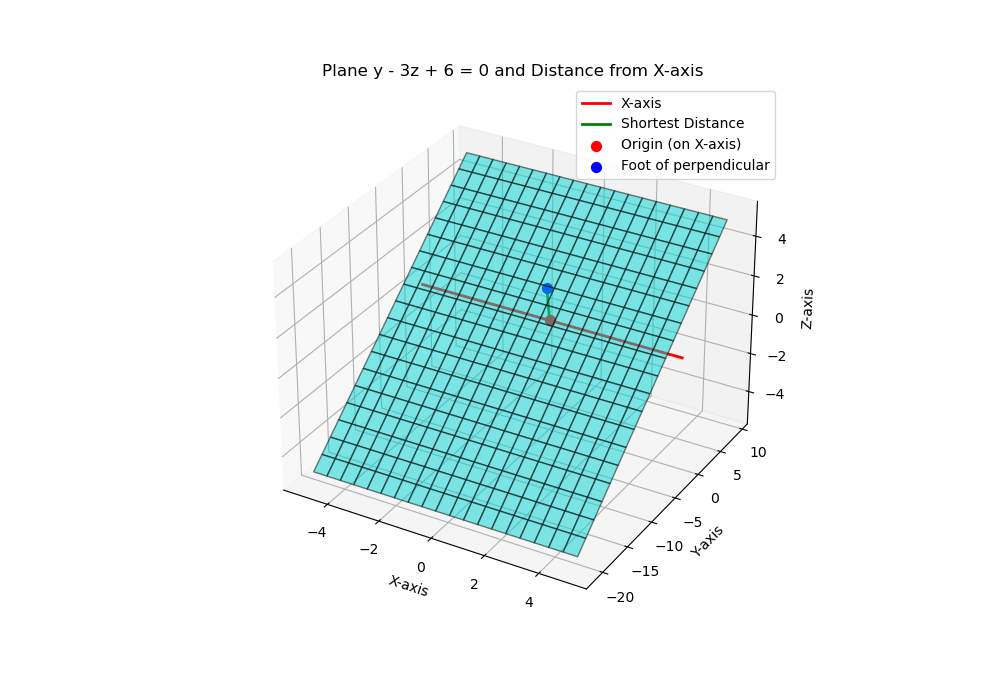
\includegraphics[width=\columnwidth, height=0.8\textheight, keepaspectratio]{figs/fig8.png}     
\end{frame}

\begin{frame}[fragile]
\frametitle{ C Code}

\begin{lstlisting}

#include <stdio.h>
#include <math.h>

int main() {
    // Coefficients of the final plane: y - 3z + 6 = 0
    double A = 0, B = 1, C = -3, D = 6;

    double x0 = 0, y0 = 0, z0 = 0;

    double numerator = fabs(A*x0 + B*y0 + C*z0 + D);
    double denominator = sqrt(A*A + B*B + C*C);
    double distance = numerator / denominator;

    printf("Equation of the plane: y - 3z + 6 = 0\n");
    printf("Distance of plane from X-axis: %.4f\n", distance);

    return 0;
}
\end{lstlisting}

\end{frame}


\begin{frame}[fragile]
\frametitle{Python and C Code}

\begin{lstlisting}

import ctypes
import numpy as np
import matplotlib.pyplot as plt
from mpl_toolkits.mplot3d import Axes3D


lib = ctypes.CDLL("./libplane.so")

# Variables to store plane coefficients
a = ctypes.c_double()
b = ctypes.c_double()
c = ctypes.c_double()
d = ctypes.c_double()
\end{lstlisting}

\end{frame}

\begin{frame}[fragile]
\frametitle{Python and C Code}

\begin{lstlisting}

# Call the C function to get coefficients
lib.get_plane(ctypes.byref(a), ctypes.byref(b), ctypes.byref(c), ctypes.byref(d))

# Extract values
a, b, c, d = a.value, b.value, c.value, d.value
print(f"Plane equation: {a}x + {b}y + {c}z + {d} = 0")


x = np.linspace(-5, 5, 30)   # X range
z = np.linspace(-5, 5, 30)   # Z range
X, Z = np.meshgrid(x, z)

# Solve plane eqn for Y:  y = (-ax - cz - d)/b
Y = (-a*X - c*Z - d) / b

\end{lstlisting}

\end{frame}

\begin{frame}[fragile]
\frametitle{Python and C Code}

\begin{lstlisting}
fig = plt.figure(figsize=(8,6))
ax = fig.add_subplot(111, projection="3d")

ax.plot_surface(X, Y, Z, alpha=0.5, color="cyan", label="Plane")

ax.plot([-5, 5], [0, 0], [0, 0], color="red", linewidth=3, label="X-axis")

# Take a point on X-axis (0,0,0)
P = np.array([0,0,0])

# Formula: foot of perpendicular from point to plane
num = a*P[0] + b*P[1] + c*P[2] + d
den = a*a + b*b + c*c

Px = P[0] - a*num/den
Py = P[1] - b*num/den
Pz = P[2] - c*num/den
\end{lstlisting}

\end{frame}

\begin{frame}[fragile]
\frametitle{Python and C Code}

\begin{lstlisting}

# Plot distance line
ax.plot([P[0], Px], [P[1], Py], [P[2], Pz],
        color="black", linewidth=3, label="Shortest distance")

# Mark points
ax.scatter(P[0], P[1], P[2], color="red", s=50, label="Origin (on X-axis)")
ax.scatter(Px, Py, Pz, color="blue", s=50, label="Foot on Plane")

ax.set_xlabel("X-axis")
ax.set_ylabel("Y-axis")
ax.set_zlabel("Z-axis")
ax.set_title("Plane y - 3z + 6 = 0 and Distance from X-axis")
ax.legend()

plt.show()
\end{lstlisting}

\end{frame}
\end{document}

